\documentclass[11pt,a4paper]{article}
\usepackage[danish]{babel}
\usepackage{icomma}
\usepackage{amsmath,amssymb,mathtools,bm}
\usepackage{booktabs,enumitem,graphicx,xcolor,environ}
\usepackage[hidelinks]{hyperref}
\usepackage[capitalise,nameinlink]{cleveref}
\usepackage[most]{tcolorbox}
\tcbuselibrary{skins,breakable}
\usepackage{tikz}
\usetikzlibrary{arrows.meta,calc,positioning,shapes.geometric}

\definecolor{gxu-paper}{HTML}{F7F9FB}
\definecolor{gxu-ink}{HTML}{1A1F2B}
\definecolor{gxu-inksoft}{HTML}{4A5568}
\definecolor{gxu-accent}{HTML}{58C4DD}
\definecolor{gxu-purple}{HTML}{7C5CFC}

\newif\ifshowanswers
\showanswerstrue

\newtcolorbox{prompt}{
  colback=gxu-paper,colframe=gxu-accent,boxrule=0.5pt,arc=4pt,
  left=8pt,right=8pt,top=6pt,bottom=6pt,
  fonttitle=\sffamily\small\bfseries,title=Arbejdsspørgsmål
}
\newtcolorbox{solution}{
  colback=gxu-accent!8,colframe=gxu-accent,boxrule=0.5pt,arc=4pt,
  left=8pt,right=8pt,top=6pt,bottom=6pt,
  fonttitle=\sffamily\small\bfseries,title=Facit
}
\NewEnviron{solutionc}{\ifshowanswers\begin{solution}\BODY\end{solution}\fi}
\newtcolorbox{definition}{
  colback=gxu-paper,colframe=gxu-purple,boxrule=0.8pt,arc=4pt,
  left=10pt,right=10pt,top=8pt,bottom=8pt,
  fonttitle=\sffamily\small\bfseries\color{gxu-purple},title=Definition
}

\newcommand{\kompetence}[1]{%
  \tcbset{mychip/.style={colback=gxu-accent!15,colframe=gxu-accent,boxrule=0.4pt,arc=10pt,left=6pt,right=6pt,top=3pt,bottom=3pt,fontupper=\sffamily\small}}
  \begin{tcolorbox}[mychip]#1\end{tcolorbox}\vspace{-4pt}
}

\makeatletter
\newcommand{\eq}[2]{\begin{equation}#2\tag{#1}\end{equation}}
\makeatother
\newcommand{\note}[1]{{\small\color{gxu-inksoft}\textit{#1}}\par}

\usepackage{fancyhdr}
\fancyhf{}
\fancyhead[L]{\sffamily\small\color{gxu-inksoft}GXU -- Matematik}
\fancyhead[R]{\sffamily\small\color{gxu-inksoft}Trigonometri \& Enhedscirkel}
\fancyfoot[C]{\thepage}
\pagestyle{fancy}
\addtolength{\textheight}{2cm}
\addtolength{\topmargin}{-1cm}

\begin{document}
\section{1. Enhedscirklen}

\kompetence{Tankegang} \kompetence{Modellering} \kompetence{Repraesentation}

\begin{figure}[ht]
\centering
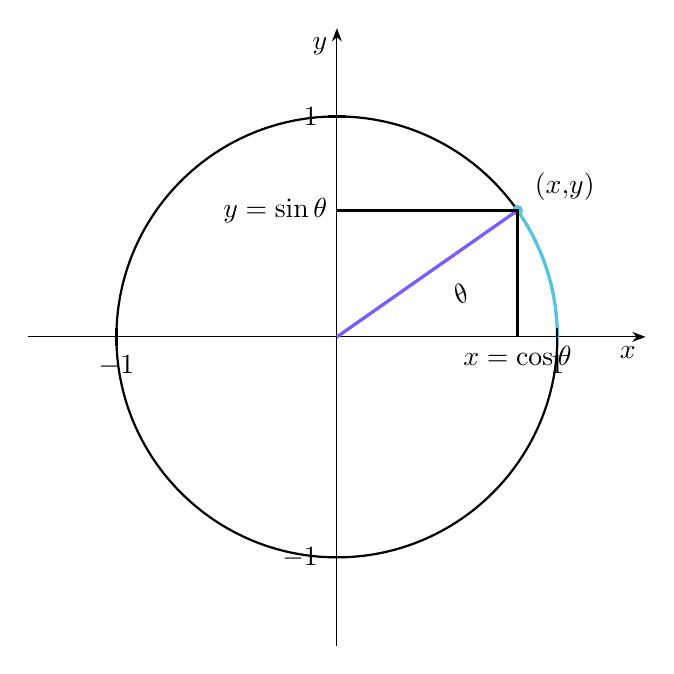
\begin{tikzpicture}[>=Stealth,scale=2.8]
  % Koordinatsystem
  \draw[->] (-1.4,0) -- (1.4,0) node[below left] {$x$};
  \draw[->] (0,-1.4) -- (0,1.4) node[below left] {$y$};
  \draw[thick] (0,0) circle (1);

  % Vinkelpunkt og sti
  \coordinate (P) at ({cos(35)},{sin(35)});
  \coordinate (Px) at ({cos(35)},0);
  \coordinate (Py) at (0,{sin(35)});

  % Vinkelbuen
  \draw[very thick,gxu-accent] (1,0) arc[start angle=0,end angle=35,radius=1];

  % Koordinat-ticks
  \foreach \t/\lab in {1/{1},-1/{-1}} {
    \draw[thick] (\t,0.04) -- (\t,-0.04) node[below] {$\lab$};
    \draw[thick] (0.04,\t) -- (-0.04,\t) node[left] {$\lab$};
  }

  % Punktet P med kryds
  \fill[gxu-accent] (P) circle (0.025);
  \node[anchor=south west] at (P) {$\;(x,y)$};

  % Projektioner (stiplede)
  \draw[dashed,gxu-inksoft] (P) -- (Px);
  \draw[dashed,gxu-inksoft] (P) -- (Py);

  % Aksel-navne ved projektionerne
  \node[below] at (Px) {$x=\cos\theta$};
  \node[left] at (Py) {$y=\sin\theta$};

  % Vinkelhældning
  \node[anchor=south west,rotate=35] at (0.55,0.08) {$\theta$};

  % Radius-linje
  \draw[very thick,gxu-purple] (0,0) -- (P);

  % Trekant horisontal/vertikal
  \draw[thick] (Px) -- (P) -- (Py);
\end{tikzpicture}
\caption{Enhedscirklen. Punktet $P=(\cos\theta,\sin\theta)$ ligger på cirklen med radius 1. Koordinaterne er direkte læsningen af $\cos\theta$ (på $x$-aksen) og $\sin\theta$ (på $y$-aksen).}
\label{fig:enhedscirkel}
\end{figure}

\begin{prompt}
Hvad er $(\cos\theta,\sin\theta)$ for $\theta = 0^{\circ}$, $\theta = 90^{\circ}$ og $\theta = 270^{\circ}$?
\end{prompt}

\begin{solutionc}
\begin{itemize}
  \item $\theta = 0^{\circ}$: $(\cos0^{\circ},\sin0^{\circ}) = (1,0)$
  \item $\theta = 90^{\circ}$: $(\cos90^{\circ},\sin90^{\circ}) = (0,1)$
  \item $\theta = 270^{\circ}$: $(\cos270^{\circ},\sin270^{\circ}) = (0,-1)$
\end{itemize}
\end{solutionc}

\section{2. Grundrelationen $\cos^{2}\theta+\sin^{2}\theta=1$}

Af figuren har trekanten med hypotenusen $1$ kateten $\cos\theta$ og $\sin\theta$, hvoraf:

\eq{1.1}{\cos^{2}\theta+\sin^{2}\theta=1}

\begin{solutionc}
\eq{}{(\tfrac{3}{5})^{2}+(\tfrac{4}{5})^{2}=\tfrac{9}{25}+\tfrac{16}{25}=\tfrac{25}{25}=1 \qquad\checkmark}
\end{solutionc}

\section{3. Pythagoras' sætning}

\kompetence{Regning} \kompetence{Tankegang}

\begin{figure}[ht]
\centering
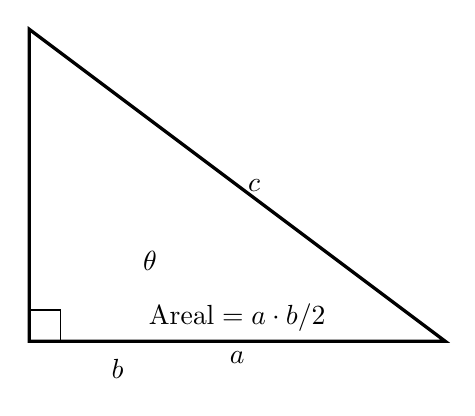
\begin{tikzpicture}[>=Stealth,scale=2.2]
  % Retvinklet trekant
  \coordinate (A) at (0,0);
  \coordinate (B) at (2.4,0);
  \coordinate (C) at (0,1.8);

  % Trekant
  \draw[very thick] (A) -- (B) node[midway,below] {$a$} -- (C) node[midway,right] {$c$} -- cycle;

  % Højre vinkel-markør
  \draw (0,0.18) -- (0.18,0.18) -- (0.18,0);

  % Vinkel-hypotenuse navn
  \node[anchor=south west] at (0.6,0.35) {$\theta$};

  % Katet-navne
  \node[below left] at (0.6,-0.05) {$b$};

  % Areal-tekster
  \node[anchor=south] at (1.2,0) {$\text{Areal}=a\cdot b/2$};
\end{tikzpicture}
\qquad
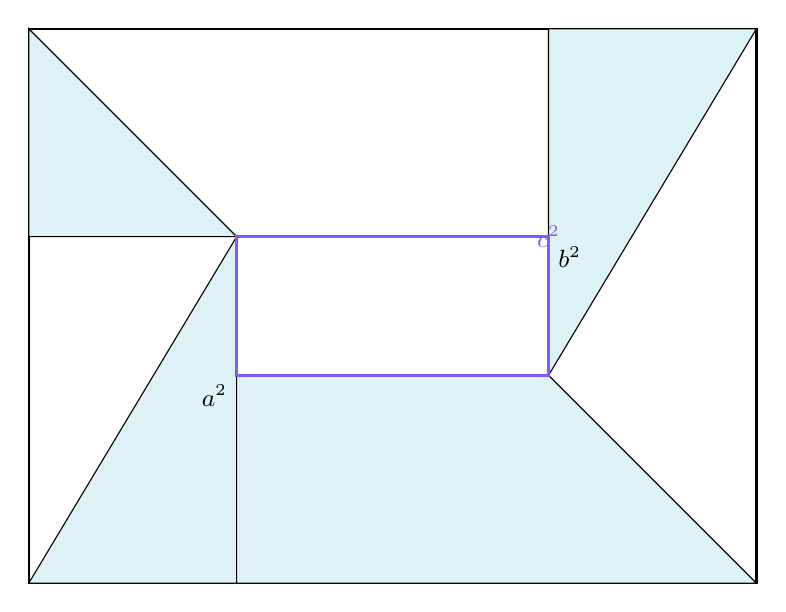
\begin{tikzpicture}[>=Stealth,scale=2.2]
  % Klassisk Pythagoras-bevis: stor kvadrat (a+b)² med fire trekanter
  % Trekant-hjørner
  \coordinate (A) at (0,0);
  \coordinate (B) at (4.2,0);
  \coordinate (C) at (4.2,3.2);
  \coordinate (D) at (0,3.2);
  % Trekanthjørner indefra
  \coordinate (T1) at (1.2,0);
  \coordinate (T2) at (4.2,1.2);
  \coordinate (T3) at (3.0,3.2);
  \coordinate (T4) at (0,2.0);
  % Diagonal kvadrat hjørner
  \coordinate (H1) at (1.2,1.2);
  \coordinate (H2) at (3.0,1.2);
  \coordinate (H3) at (3.0,2.0);
  \coordinate (H4) at (1.2,2.0);

  % Store kvadrat yderside
  \draw[thick] (A) rectangle (C);
  % Fire trekanter
  \draw[fill=gxu-accent!20] (A) -- (T1) -- (H1) -- (H4) -- cycle;
  \draw[fill=gxu-accent!20] (T1) -- (B) -- (H2) -- (H1) -- cycle;
  \draw[fill=gxu-accent!20] (H2) -- (C) -- (T3) -- (H3) -- cycle;
  \draw[fill=gxu-accent!20] (H4) -- (H3) -- (T4) -- (D) -- cycle;
  % Indre kvadrat (hypotenusen c)
  \draw[very thick,gxu-purple] (H1) -- (H2) -- (H3) -- (H4) -- cycle;
  % Areal-tekst
  \node[anchor=north east,font=\sffamily\small] at (H1) {$a^{2}$};
  \node[anchor=north west,font=\sffamily\small] at (H3) {$b^{2}$};
  \node[anchor=center,font=\sffamily\small\color{gxu-purple}] at (H2 |- H3) {$c^{2}$};
\end{tikzpicture}
\caption{Venstte: retvinklet trekant med kateter $a$ og $b$ samt hypotenuse $c$. Højre: samme trekant indlagt i et kvadrat, der viser at $a^{2}+b^{2}=c^{2}$.}
\label{fig:pythagoras}
\end{figure}

For en retvinklet trekant gælder:

\eq{3.1}{a^{2}+b^{2}=c^{2}}

hvor $c$ er hypotenusen (den længste side, modsat den rette vinkel).

\begin{prompt}
En retvinklet trekant har kateter $a=3$ og $b=4$. Find hypotenusen $c$.
\end{prompt}
\begin{solutionc}
$c^{2}=3^{2}+4^{2}=9+16=25$, så $c=5$.
\end{solutionc}

\section{4. Sinus, cosinus og tangens}

\kompetence{Regning} \kompetence{Modellering} \kompetence{Hjaelpemidler}

\begin{figure}[ht]
\centering
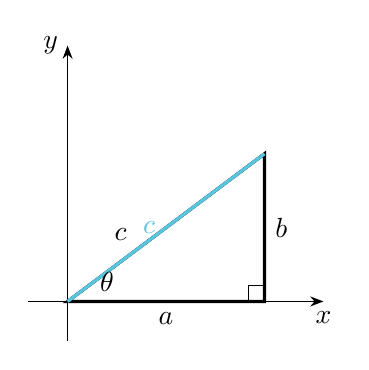
\begin{tikzpicture}[>=Stealth,scale=2.5]
  % Koordinatsystem
  \draw[->] (-0.2,0) -- (1.3,0) node[below] {$x$};
  \draw[->] (0,-0.2) -- (0,1.3) node[left] {$y$};

  % Trekant
  \coordinate (A) at (0,0);
  \coordinate (B) at (1,0);
  \coordinate (C) at (1,0.75);

  % Trekant-sider
  \draw[very thick] (A) -- (B) node[midway,below] {$a$} -- (C) node[midway,right] {$b$} -- cycle;
  \draw[very thick,gxu-accent] (A) -- (C) node[midway,left] {$c$};

  % Vinkel
  \node at (0.2,0.1) {$\theta$};

  % Ret vinkel-markør
  \draw (0.92,0) -- (0.92,0.08) -- (1,0.08);

  % Hypotenuse-navn flyttet
  \node[anchor=south east] at (0.35,0.26) {$c$};
\end{tikzpicture}
\qquad
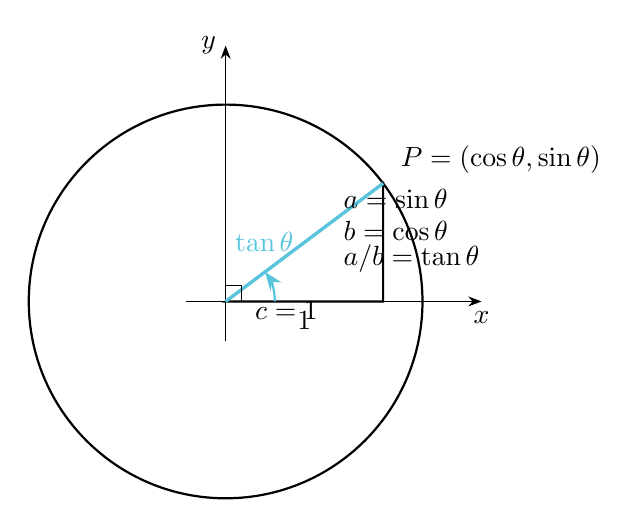
\begin{tikzpicture}[>=Stealth,scale=2.5]
  \pgfmathsetmacro{\cx}{cos(36.87)}
  \pgfmathsetmacro{\cy}{sin(36.87)}
  % Koordinatsystem
  \draw[->] (-0.2,0) -- (1.3,0) node[below] {$x$};
  \draw[->] (0,-0.2) -- (0,1.3) node[left] {$y$};
  \draw[thick] (0,0) circle (1);

  % Trekant: ret vinkel ved O, hypotenuse = radius til P
  \coordinate (P) at (\cx,\cy);
  \coordinate (B) at (\cx,0);
  \draw[thick] (0,0) -- (B) node[midway,below] {$1$} -- (P) -- cycle;
  \draw[very thick,gxu-accent] (0,0) -- (P) node[midway,left] {$\tan\theta$};

  % Ret vinkel-markør ved O
  \draw (0.08,0) -- (0.08,0.08) -- (0,0.08);

  % Radius = 1 label
  \node[anchor=north west] at (0.1,0.05) {$c=1$};

  % Vinkel-buе med pil
  \draw[->,thick,gxu-accent] (0.25,0) arc[start angle=0,end angle=36.87,radius=0.25];

  % Tekst
  \node[anchor=south west] at (0.55,0.10) {$a/b = \tan\theta$};
  \node[anchor=south west] at (0.55,0.26) {$b = \cos\theta$};
  \node[anchor=south west] at (0.55,0.42) {$a = \sin\theta$};

  % Navn P
  \node[anchor=south west] at (\cx+0.04,\cy) {$P=(\cos\theta,\sin\theta)$};
\end{tikzpicture}
\caption{Venstte: sinus, cosinus og tangens defineret fra en retvinklet trekant. Højre: de samme forhold aflæst på enhedscirklen.}
\label{fig:trigtrekant}
\end{figure}

For en retvinklet trekant med vinkel $\theta$ gælder:

\eq{4.1}{\sin\theta=\frac{a}{c}\qquad\cos\theta=\frac{b}{c}\qquad\tan\theta=\frac{a}{b}}

hvor $a$ er kateten over for $\theta$, $b$ er kateten hos $\theta$, og $c$ er hypotenusen.

\note{Vinklen $\theta$ er i grader.}

\begin{prompt}
I en retvinklet trekant er $a=5$ og $c=13$. Find $\sin\theta$, $\cos\theta$ og $\tan\theta$.
\end{prompt}
\begin{solutionc}
Først $b=\sqrt{13^{2}-5^{2}}=\sqrt{169-25}=\sqrt{144}=12$.\\
Derefter: $\sin\theta=5/13$, $\cos\theta=12/13$, $\tan\theta=5/12$.
\end{solutionc}

\section{5. Opgaver}

\kompetence{Regning} \kompetence{Tankegang} \kompetence{Hjaelpemidler}

\noindent\textbf{Regel for alle opgaver:} hver opgave giver præcis to informationer -- enten to sider ($a$, $b$, $c$) eller en vinkel ($\theta$) og en side. Løs for den ukendte størrelse.

\subsection*{Type A -- Pythagoras: to kendte sider, find den tredje}

\begin{enumerate}

\item
Givet $a=6$ og $b=8$. Find $c$.
\begin{solutionc}
$c=\sqrt{6^{2}+8^{2}}=\sqrt{36+64}=\sqrt{100}=10$.
\end{solutionc}

\item
Givet $a=5$ og $c=13$. Find $b$.
\begin{solutionc}
$b=\sqrt{13^{2}-5^{2}}=\sqrt{169-25}=\sqrt{144}=12$.
\end{solutionc}

\item
Givet $b=9$ og $c=15$. Find $a$.
\begin{solutionc}
$a=\sqrt{15^{2}-9^{2}}=\sqrt{225-81}=\sqrt{144}=12$.
\end{solutionc}

\item
Givet $a=20$ og $b=21$. Find $c$.
\begin{solutionc}
$c=\sqrt{20^{2}+21^{2}}=\sqrt{400+441}=\sqrt{841}=29$.
\end{solutionc}

\end{enumerate}

\subsection*{Type B -- Trigonometri: en vinkel og en side, find de to andre sider}

\begin{enumerate}[resume]

\item
Givet $\theta=30^{\circ}$ og $c=10$. Find $a$ og $b$.
\begin{solutionc}
$a=c\sin\theta=10\cdot\tfrac{1}{2}=5$. \quad $b=c\cos\theta=10\cdot\tfrac{\sqrt{3}}{2}=5\sqrt{3}\approx8{,}66$.
\end{solutionc}

\item
Givet $\theta=60^{\circ}$ og $a=7$. Find $b$ og $c$.
\begin{solutionc}
$\tan60^{\circ}=\sqrt{3}\Rightarrow b=a/\tan\theta=7/\sqrt{3}\approx4{,}04$. \quad $c=a/\sin\theta=7/(\sqrt{3}/2)=14/\sqrt{3}\approx8{,}08$.
\end{solutionc}

\item
Givet $\theta=45^{\circ}$ og $c=12$. Find $a$ og $b$.
\begin{solutionc}
$a=b=c\sin45^{\circ}=12\cdot\tfrac{\sqrt{2}}{2}=6\sqrt{2}\approx8{,}49$. \quad $b=a\approx8{,}49$.
\end{solutionc}

\item
Givet $\theta=53{,}13^{\circ}$ og $b=12$. Find $a$ og $c$.
\begin{solutionc}
$\tan53{,}13^{\circ}=4/3\Rightarrow a=b\tan\theta=12\cdot\tfrac{4}{3}=16$. \quad $c=\sqrt{a^{2}+b^{2}}=\sqrt{256+144}=\sqrt{400}=20$.
\end{solutionc}

\end{enumerate}

\subsection*{Type C -- Beviser og aflæsning}

\begin{enumerate}[resume]

\item
Bevis grundrelationen $\cos^{2}\theta+\sin^{2}\theta=1$ ud fra en retvinklet trekant
med $\sin\theta=a/c$ og $\cos\theta=b/c$.
\begin{solutionc}
$(a/c)^{2}+(b/c)^{2}=(a^{2}+b^{2})/c^{2}=c^{2}/c^{2}=1$ ved Pythagoras.
\end{solutionc}

\item
Vis at $(3/5,4/5)$ ligger på enhedscirklen.
\begin{solutionc}
$(\tfrac{3}{5})^{2}+(\tfrac{4}{5})^{2}=\tfrac{9}{25}+\tfrac{16}{25}=\tfrac{25}{25}=1$ $\checkmark$.
\end{solutionc}

\end{enumerate}

\end{document}
